\subsection*{Problema 01}

\noindent \textbf{Enunciado:} \\
Calcular la integral indefinida:
\begin{align*}
\int \dfrac{dx}{4x^2 + 4x + 10}
\end{align*}

\noindent \textbf{Solución:} \\
Primero, analizamos el denominador de la función integranda. Completamos el trinomio cuadrado perfecto agrupando los términos en $x$:
\begin{align*}
4x^2 + 4x + 10 &= 4\left(x^2 + x\right) + 10
\end{align*}

\noindent Completamos el cuadrado dentro del paréntesis sumando y restando $\left(\frac{1}{2}\right)^2 = \frac{1}{4}$:
\begin{align*}
4x^2 + 4x + 10 &= 4\left(x^2 + x + \dfrac{1}{4} - \dfrac{1}{4}\right) + 10 \\
&= 4\left(x + \dfrac{1}{2}\right)^2 - 1 + 10 \\
&= 4\left(x + \dfrac{1}{2}\right)^2 + 9
\end{align*}

\noindent Sustituimos esta expresión equivalente en el denominador de la integral original:
\begin{align*}
\int \dfrac{dx}{4x^2 + 4x + 10} &= \int \dfrac{dx}{4\left(x + \frac{1}{2}\right)^2 + 9}
\end{align*}

\noindent Para resolver esta integral, aplicamos la sustitución trigonométrica sugerida o un cambio de variable lineal. Sea:
\begin{align*}
u &= x + \dfrac{1}{2}, \quad du = dx
\end{align*}

\noindent La integral se transforma en:
\begin{align*}
\int \dfrac{du}{4u^2 + 9} &= \int \dfrac{du}{9 \left(\left(\frac{2}{3}u\right)^2 + 1\right)}
\end{align*}

\noindent Hacemos un segundo cambio de variable con $w = \frac{2}{3}u$, de donde $dw = \frac{2}{3}du$, lo que implica $du = \frac{3}{2}dw$:
\begin{align*}
&= \dfrac{1}{9} \int \dfrac{\frac{3}{2} dw}{w^2 + 1} \\
&= \dfrac{3}{18} \int \dfrac{dw}{w^2 + 1} \\
&= \dfrac{1}{6} \arctan(w) + C
\end{align*}

\noindent Retornando a la variable original $u$ y posteriormente a $x$:
\begin{align*}
&= \dfrac{1}{6} \arctan\left(\dfrac{2}{3}u\right) + C \\
&= \dfrac{1}{6} \arctan\left[\dfrac{2}{3}\left(x + \dfrac{1}{2}\right)\right] + C \\
&= \dfrac{1}{6} \arctan\left(\dfrac{2x + 1}{3}\right) + C
\end{align*}

\noindent Por lo tanto, el resultado de la integral indefinida es:
\begin{align*}
\int \dfrac{dx}{4x^2 + 4x + 10} = \dfrac{1}{6} \arctan\left(\dfrac{2x + 1}{3}\right) + C
\end{align*}

\begin{figure}[H]
	\centering
	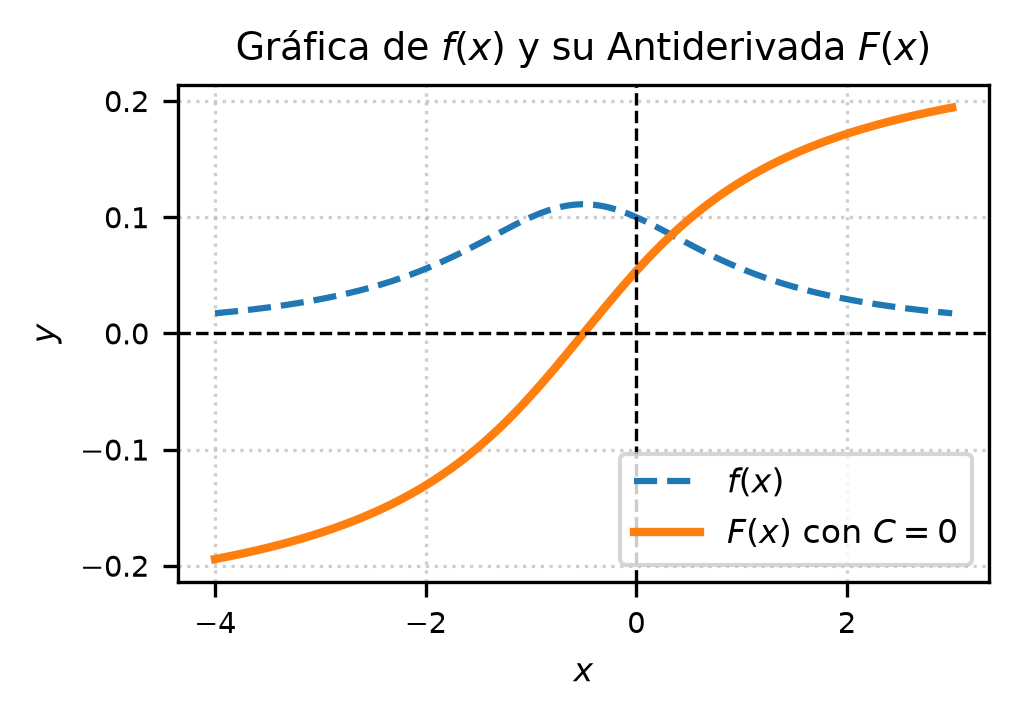
\includegraphics[width=\columnwidth]{semana_03/graficas/SEM03_P01_grafica.png}
	\caption{Representación gráfica de $f(x)$ y su antiderivada $F(x)$ evaluada para la constante de integración $C = 0$ (Problema 01).}
	\label{fig:problema01}
\end{figure}
